\chapter{PCB Design}
\label{cap:pcbdesign}

Following the initial development on a breadboard, the natural progression in the design evolution was to 
transition to a perfboard assembly. This intermediate step not only served to condense the device's 
footprint but also offered a preliminary glimpse into its form and functionality. Subsequently, the 
culmination of this iterative process involved the design and fabrication of a PCB tailored to the 
project's specifications, marking a significant milestone in its realization.


\section{Assembling on a Perfboard}

Perfboards, short for perforated boards, are commonly used prototyping platforms in electronics. They 
consist of a board with a grid of holes spaced at regular intervals. These holes are surrounded by copper 
pads or traces that can be connected using solder to create electronic circuits. Perfboards allow 
electronic components, such as resistors, capacitors, integrated circuits, and other discrete components, 
to be soldered onto the board, facilitating the creation of temporary or semi-permanent circuits for 
testing and development purposes \cite{perfboard}. They serve as a practical and versatile tool for 
electronics hobbyists, engineers, and designers to quickly prototype and iterate on circuit designs 
before moving to more permanent solutions like printed circuit boards (PCBs). Examples can be seen in 
Figures \ref{fig:perfboard_assembled_back} and \ref{fig:perfboard_assembled_front}.

In the context of this project, transitioning to a perfboard prototype served multiple crucial purposes. 
Firstly, it offered a tangible visualization of the future device's physical footprint, providing 
executives with a concrete representation of the project's direction and potential. This visual aid not 
only conveyed the scale and form of the device but also showed its feasibility and progress, instilling 
confidence in its development trajectory.

To commence this phase, a diagram detailing the placement of each component and its connection to the 
corresponding pins on the microcontroller was drafted. This diagram served as a blueprint, guiding the 
subsequent assembly process.

With the schematic as a roadmap, the assembly of the perfboard prototype commenced. Components were 
transitioned from the breadboard to the perfboard, ensuring each element found its designated place. 
Careful consideration was given to the layout, optimizing spatial organization for efficient circuitry 
and minimal interference.

\begin{figure}[h]
    \centering
    \begin{minipage}[b]{0.45\textwidth}
        \centering
        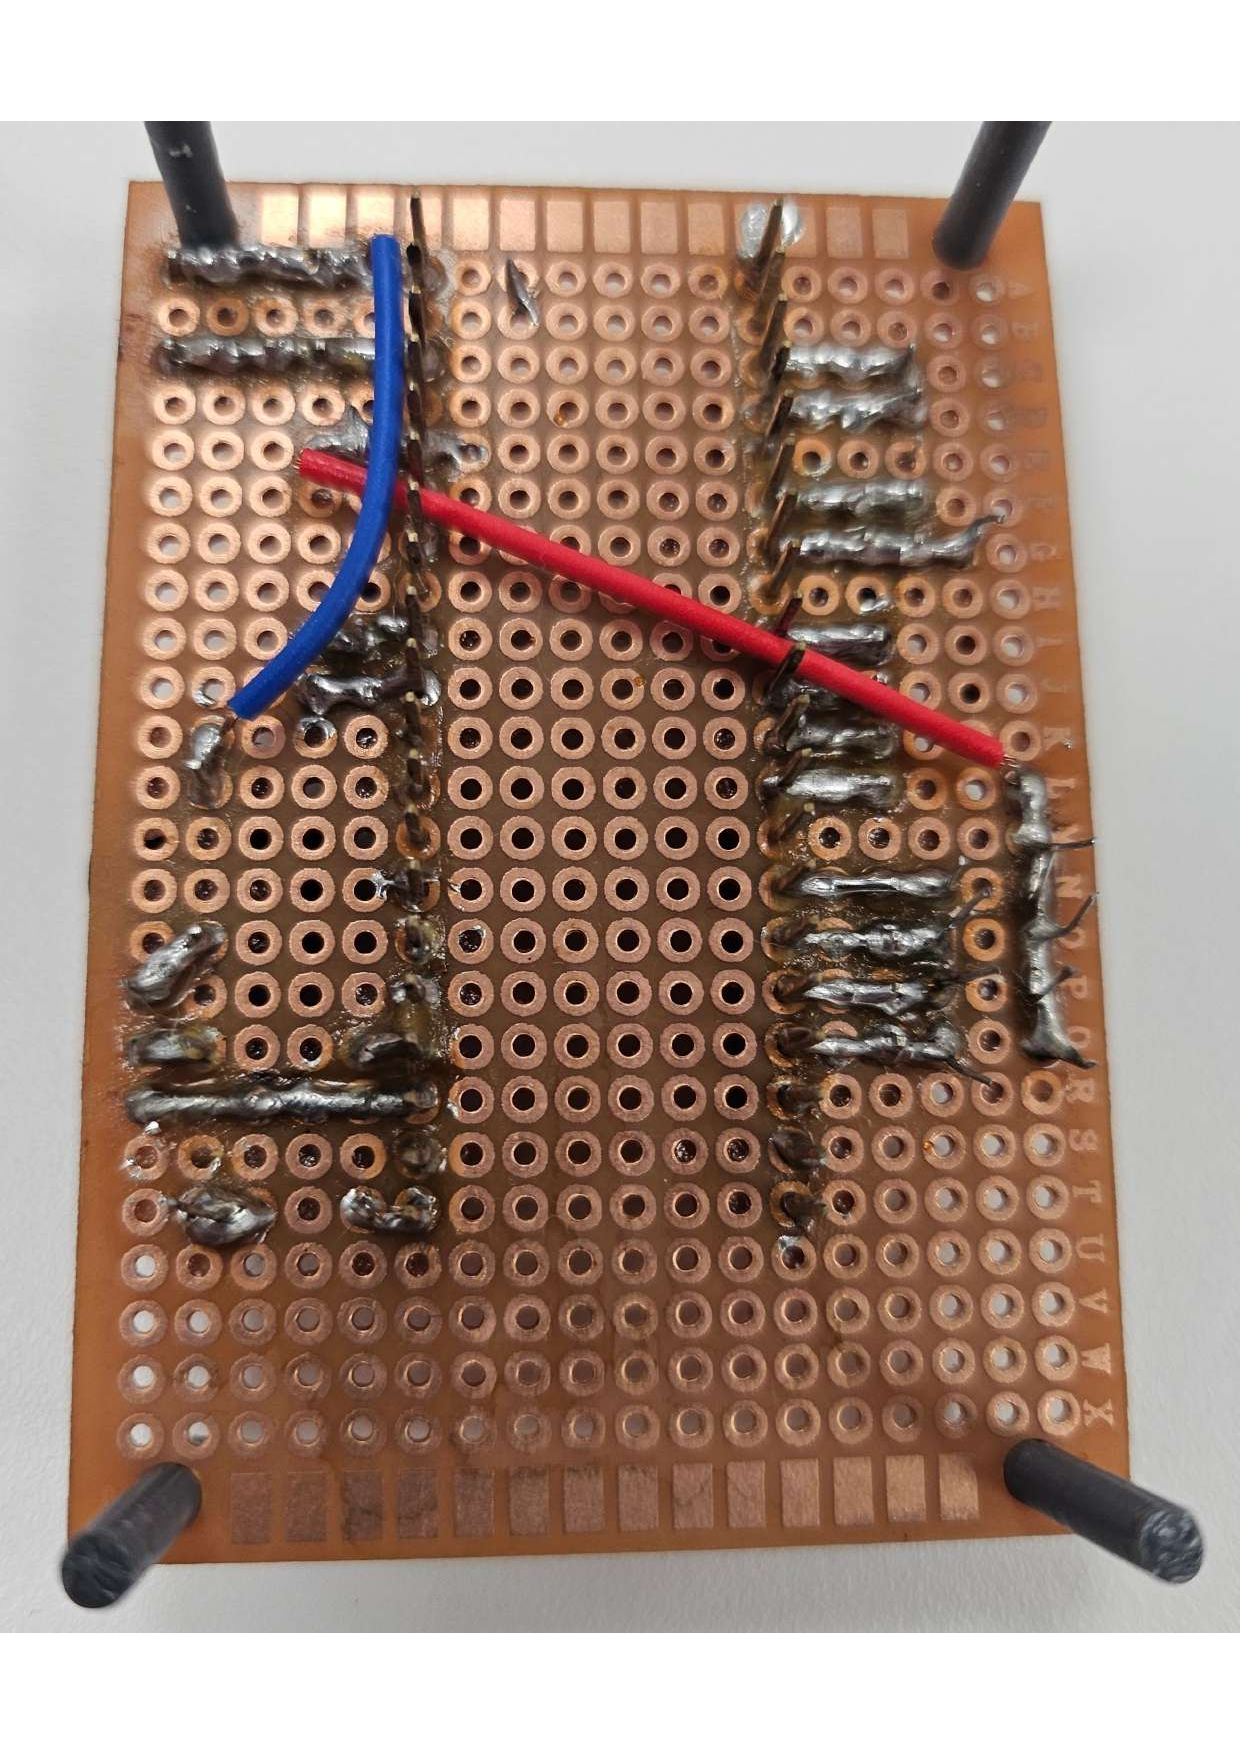
\includegraphics[width=.8\textwidth]{Imagenes/Vectorial/perfboard_assembled_back.pdf}
        \caption{Back side of the assembled perfboard}
        \label{fig:perfboard_assembled_back}
    \end{minipage}
    \hfill
    \begin{minipage}[b]{0.45\textwidth}
        \centering
        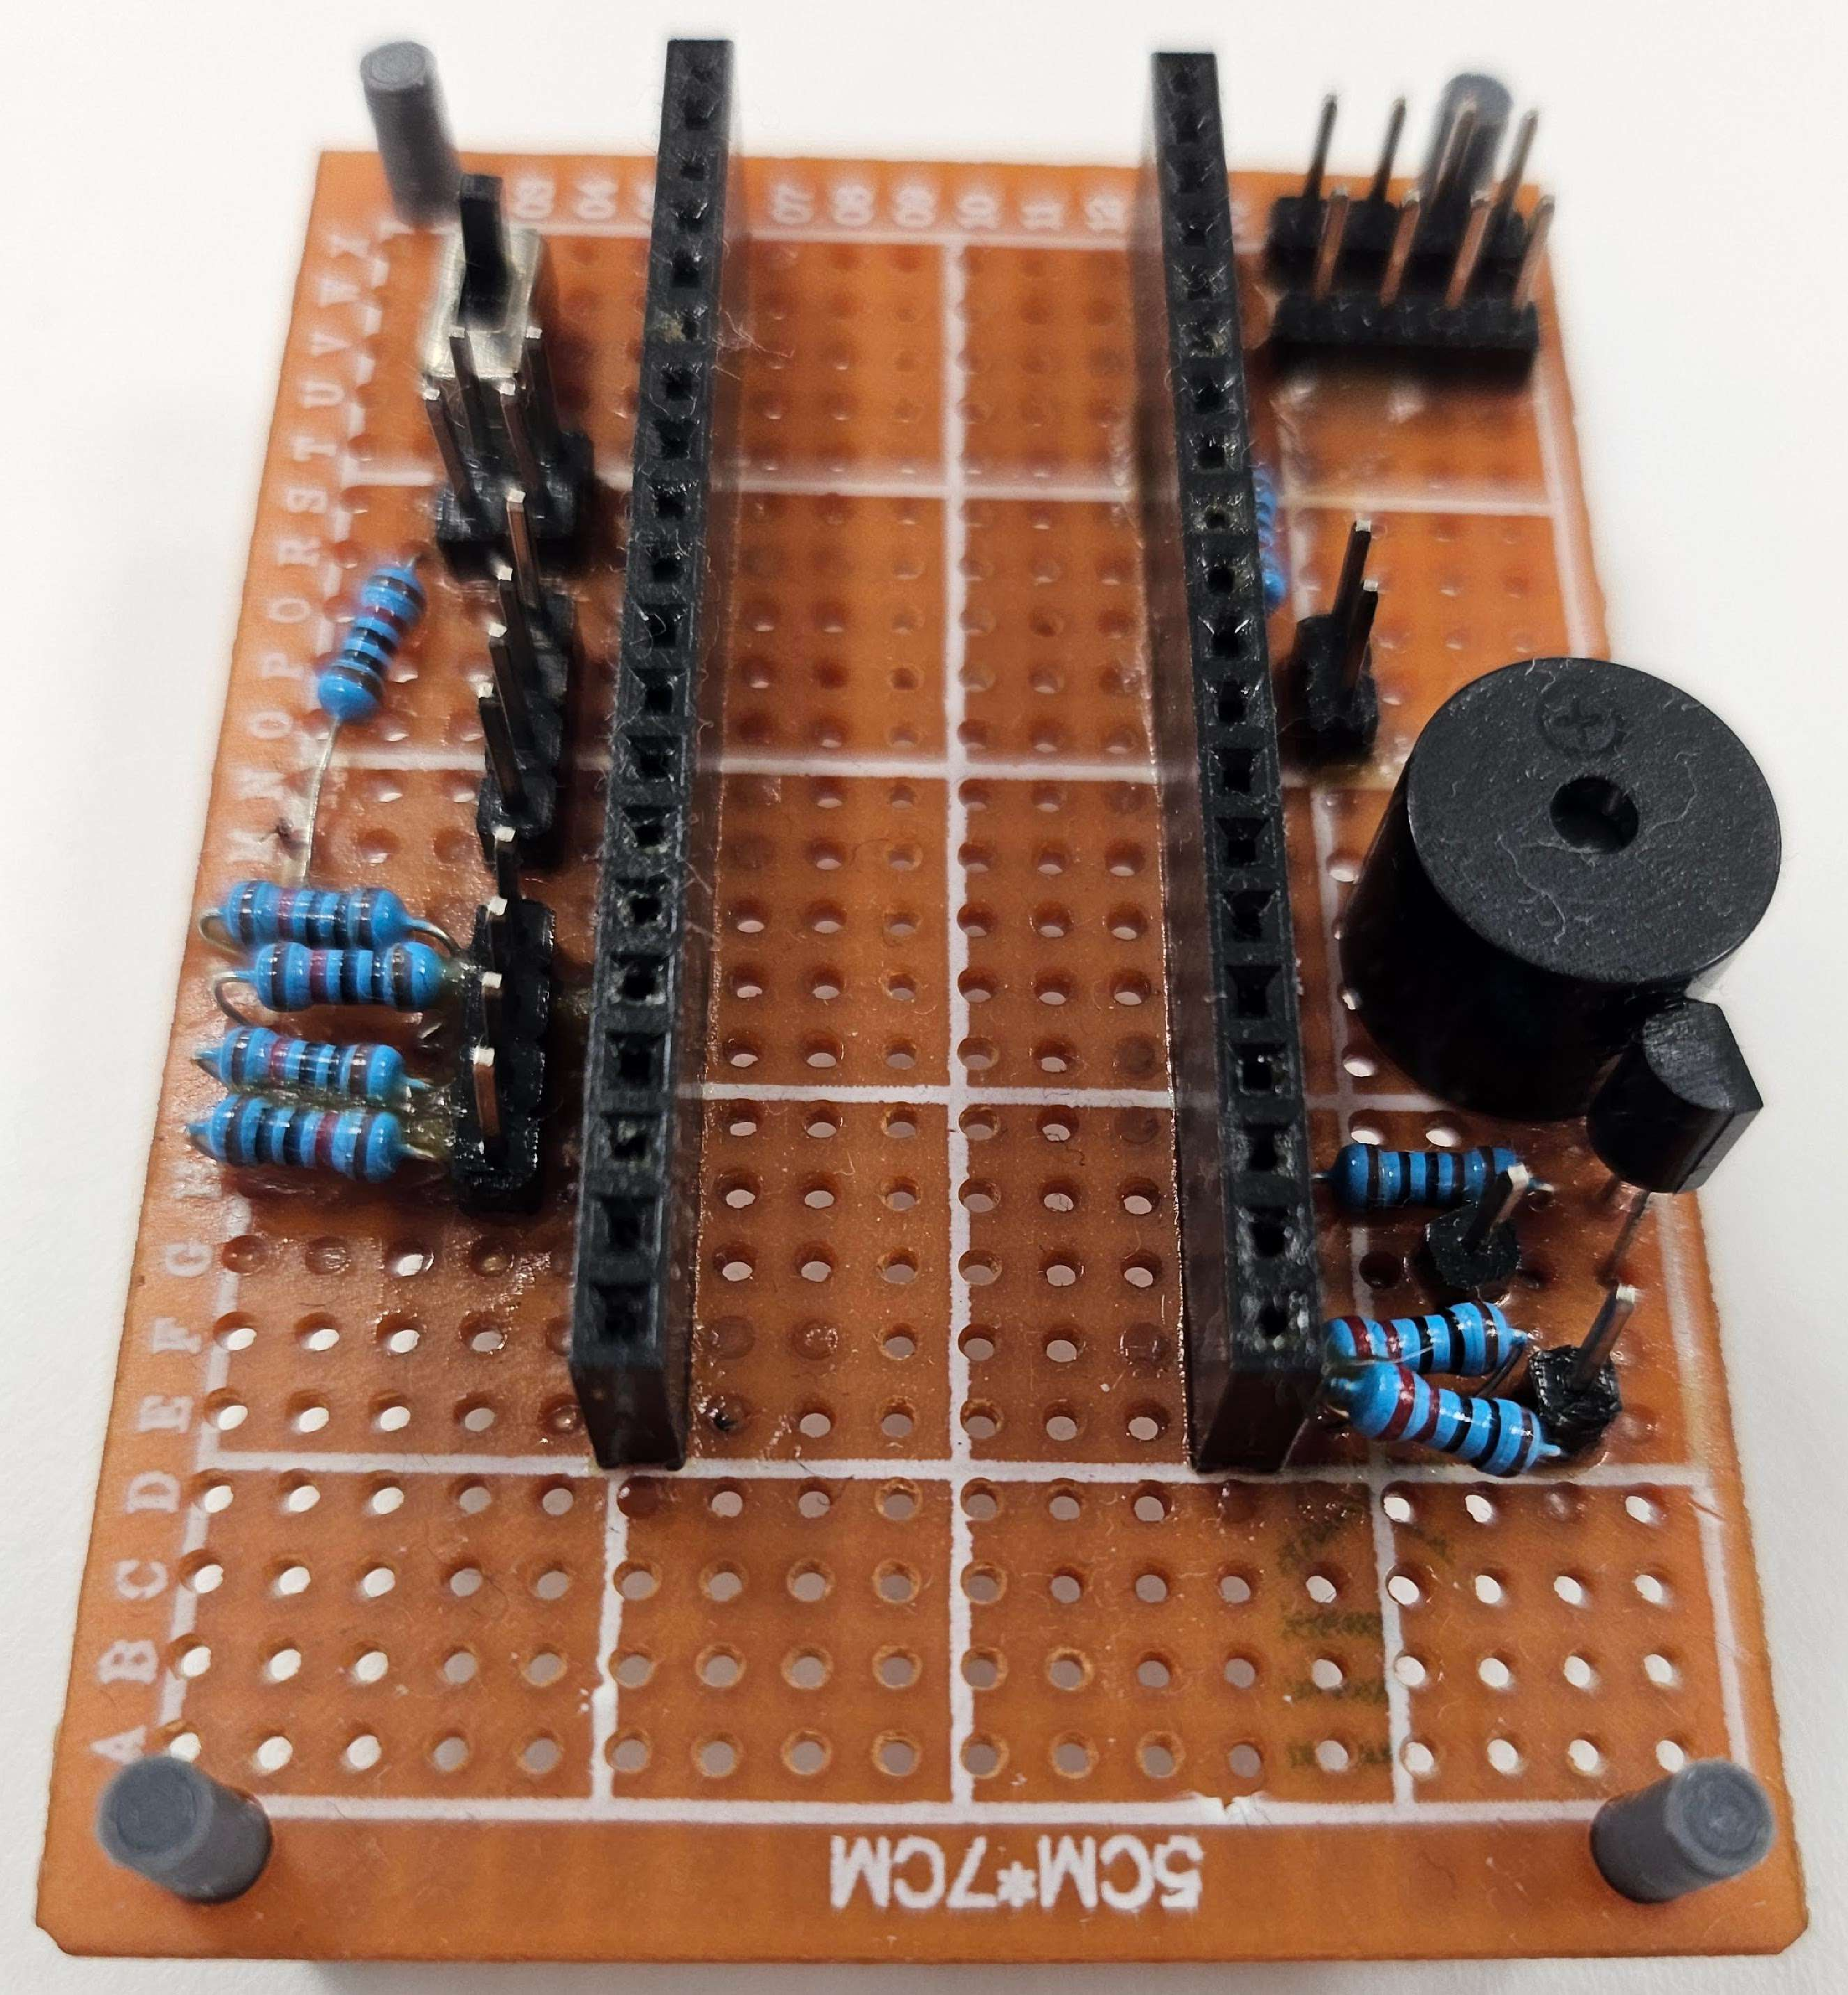
\includegraphics[width=.8\textwidth]{Imagenes/Vectorial/perfboard_assembled_front.pdf}
        \caption{Front side of the assembled perfboard}
        \label{fig:perfboard_assembled_front}
    \end{minipage}
\end{figure}


\section{Designing the PCB}

Now that the perfboard provided a good idea of how the PCB would be, now it has to be properly designed. 
As it could be seen before, the perfboard's main job was to bring all components together, and that will 
also be the case for the PCB. It would give a much cleaner look than the perfboard, and be much more 
comfortable to plug components into, since on the perfboard traces could not overlap, limiting design 
possibilities. Now, with a multi-layer PCB, traces could go above and below each other, allowing for the 
placement continuous male headers for each component.

Having used the perfboard as a preliminary platform to consolidate components and understand the spatial 
dynamics of the circuit, the focus now shifts towards the meticulous design of the printed circuit board 
(PCB).

The primary function of the PCB mirrors that of the perfboard: to integrate and interconnect all 
components seamlessly. However, unlike the perfboard, the PCB offers advantages in terms of aesthetics, 
functionality, and ease of assembly.

Moreover, the transition to a multi-layer PCB introduces a realm of design possibilities previously 
unattainable with the perfboard. By using multiple layers, traces can now traverse both above and below 
the surface, allowing for more flexibility in component placement and routing. This feature allows for 
the implementation of continuous male headers for each component, which were not easily implemented with 
the perfboard.


\subsection{Requirements}

As mentioned earlier, this PCB is designed primarily as an interconnection platform for the various 
components of the device, making its complexity relatively low.

The SIM7020E board would be positioned beneath the Pi Pico using stacking headers, as illustrated in 
Figure \ref{fig:sim7020e_topview}, thereby reducing the number of interconnections required. 

Additionally, it requires integration of the buzzer and its transistor, while certain parts were retained 
in case of future requirements, given their minimal cost. These include the matrix keyboard's header, the 
additional NFC reader's header, and the LED's header. Further details on the cost will be provided in the 
next section.

Another critical requirement driving the development of a custom PCB is the need to streamline the 
device's assembly processes. In line with this objective, it's essential for the PCB to arrive 
pre-assembled. While it's common for boards to be sold without soldered components, pre-assembled PCBs are 
a must for this project to be economically and logistically viable. Thus, an ideal provider would offer 
both manufacturing and assembly services.


\subsection{Design and Production}

In the quest for a user-friendly PCB design program, \textit{EasyEDA}\footnote{EasyEDA's website: 
\url{https://easyeda.com/}} emerged as a promising option. Offering a schematic design tool, it facilitated 
the transition from hand-drawn schematics to digital diagrams. EasyEDA allows users to seamlessly translate 
these diagrams into PCB layouts, enabling the placement of components, definition of board dimensions, and 
automatic routing of traces to interconnect all elements. Thanks to its simplicity, a final design was 
swiftly achieved within a matter of days.

It was discovered that EasyEDA has a partnership with \textit{JLCPCB}\footnote{JLCPCB's website: 
\url{https://jlcpcb.com/}}, a company offering comprehensive PCB manufacturing and assembly services. 
Additionally, EasyEDA seamlessly integrates with \textit{LCSC}\footnote{LCSC's website: 
\url{https://www.lcsc.com/}}, a supplier providing a comprehensive parts catalog with detailed specifications 
for each component used in the project. Notably, the final pricing was highly competitive, and with all these 
providers working together, support extended throughout the entire production process, from schematic design 
to the final product.

A few considerations regarding part selection:
\begin{itemize}
    \item Since active buzzers can only be turned on or off, the sound's frequency is already pre-determined. 
    This has to be taken into consideration when choosing one.
    \item The transistor responsible for controlling power to the buzzer must meet the power specifications 
    and respond to changes in voltage from a GPIO pin (3.3V). Fortunately, given that the voltage at the 
    drain is 5V and the current is in the milliamp range, virtually any transistor would be suitable for 
    this purpose.
    \item Since regular \textit{DuPont} jumper wires will be used, each one of the headers' pins have to be 
    2.54mm apart (which is the equivalent to 0.1 inches), thus compatible headers need to be selected.
    \item Mounting holes would be needed on each corner to attach it to a box, which would be designed in 
    the future.
\end{itemize}

After navigating through a learning curve with the parts catalogue and sorting through dozens of providers 
for each component, all necessary parts were successfully chosen, and the PCB was prepared for production.

\begin{figure}[h]
    \centering
    \begin{minipage}[b]{0.45\textwidth}
        \centering
        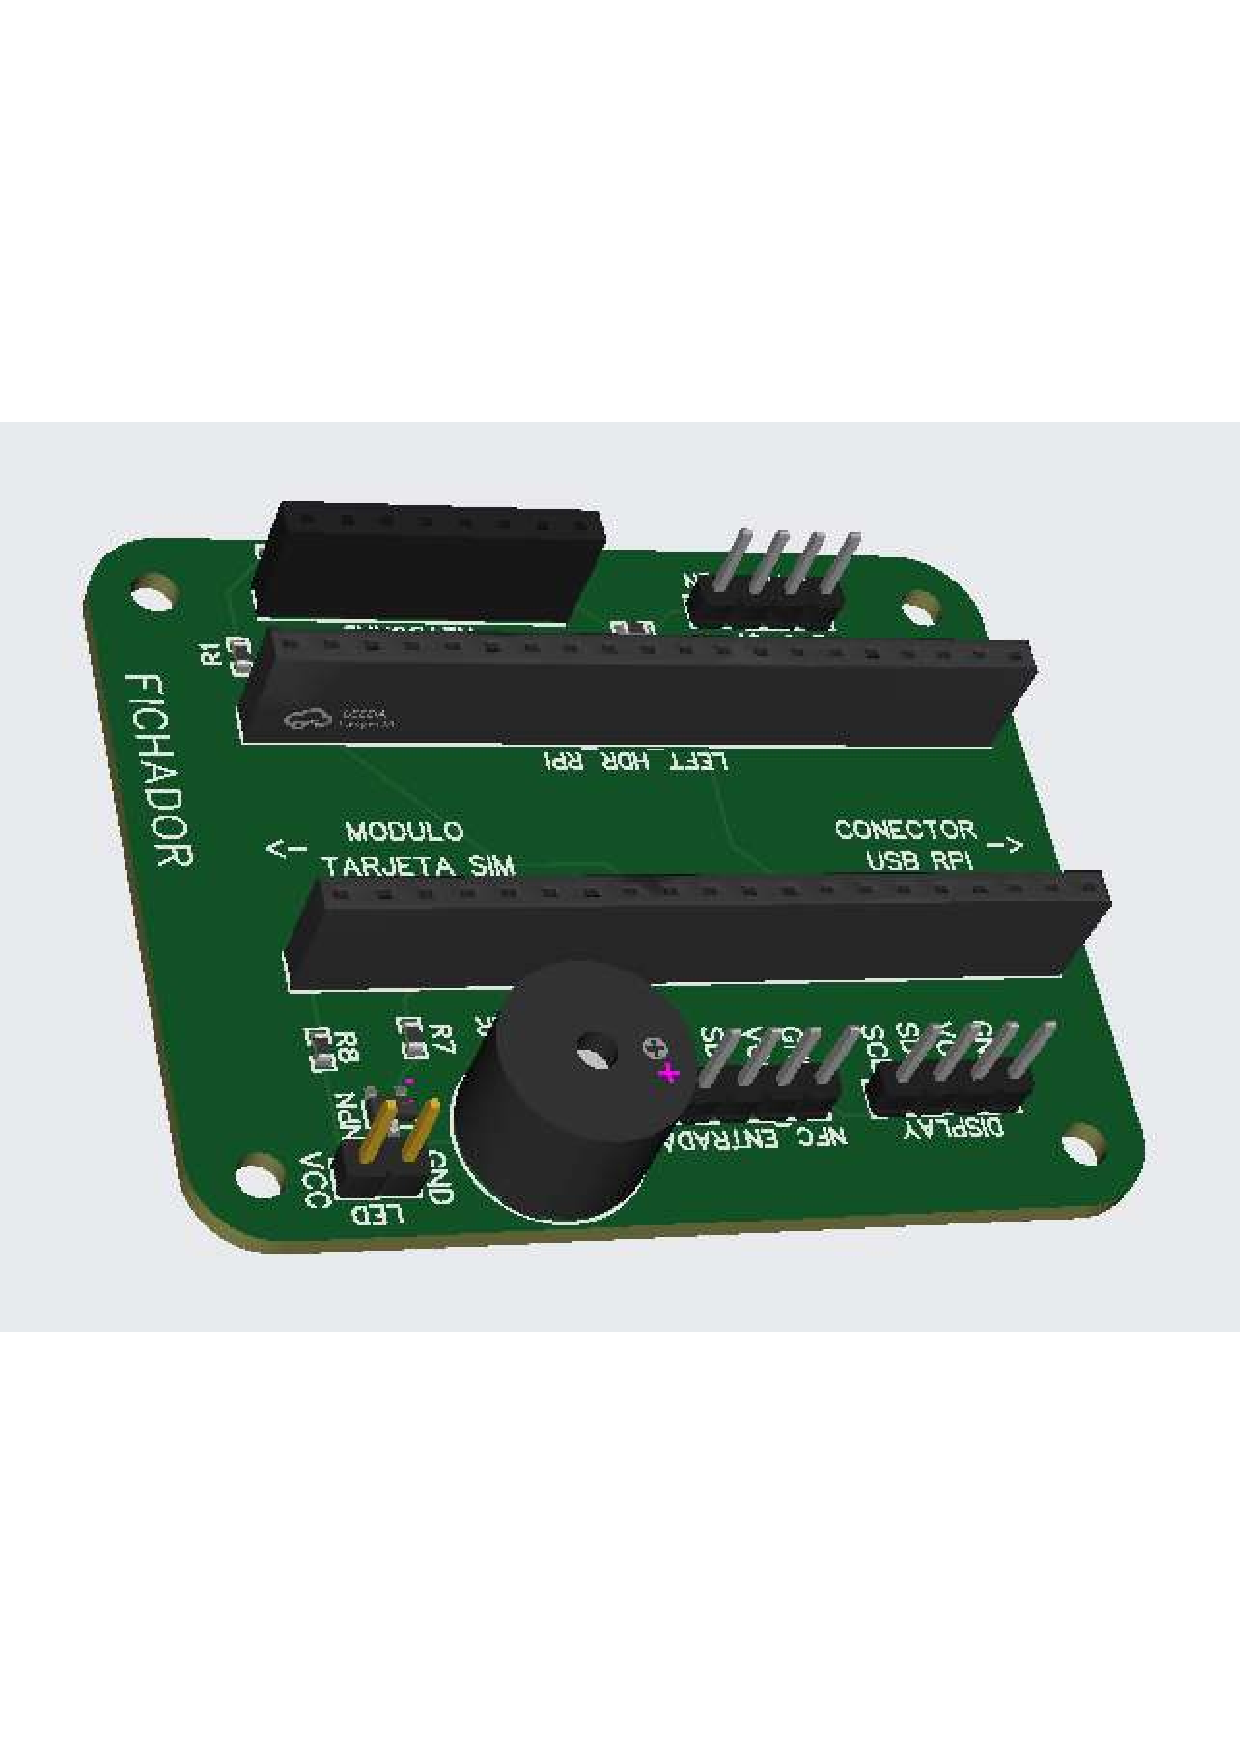
\includegraphics[width=.9\textwidth]{Imagenes/Vectorial/pcb1.pdf}
        \caption{PCB's top view}
        \label{fig:pcb_topview}
    \end{minipage}
    \hfill
    \begin{minipage}[b]{0.45\textwidth}
        \centering
        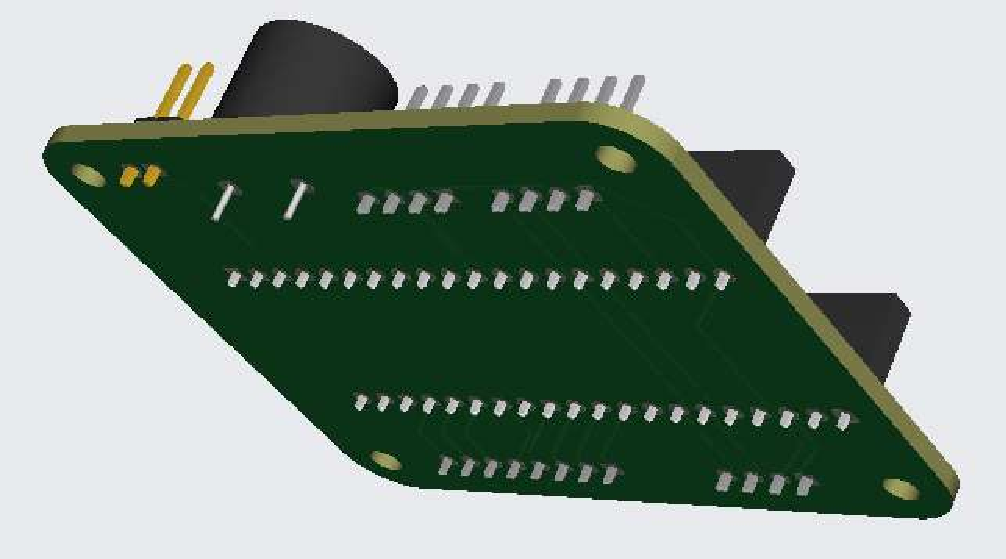
\includegraphics[width=.9\textwidth]{Imagenes/Vectorial/pcb2.pdf}
        \caption{PCB's bottom view}
        \label{fig:pcb_bottomview}
    \end{minipage}
\end{figure}

During the ordering process, a 3D model of the PCB with the selected parts is displayed, similar to Figures 
\ref{fig:pcb_topview} and \ref{fig:pcb_bottomview}. It's important to note that the PCBs are manufactured in 
China and then shipped internationally. Factors such as import tariffs and shipping costs need to be taken 
into account. Despite these considerations, the price remained competitive compared to local alternatives, 
even after factoring in customs duties and shipping fees. Remarkably, the PCBs arrived within a week of 
ordering.

The quality of construction exceeded expectations, with all components fitting perfectly on the first try. 
The selected buzzer emitted the expected pitch, and everything functioned as intended. Executives were 
pleasantly surprised by the remarkably low price per unit.
